\documentclass[sigconf]{acmart}

\usepackage{url}

\settopmatter{printacmref=false}

\begin{document}

\title{Movie Search Engine with Clustering}

\author{Raj Patel}
\affiliation{%
  \institution{University of Utah}
}
\email{raj.patel@utah.edu}

\author{Blaze Kotsenburg}
\affiliation{%
  \institution{University of Utah}
}
\email{bkotsenburg@gmail.com}

\author{Brandon Ward}
\affiliation{%
  \institution{University of Utah}
}
\email{brandon.ward@utah.edu}

\begin{abstract}
Our project was an exploratory project with the goal of developing a search engine based on what we have learned in class. We propose to develop a search engine for a movie dataset containing a collection of information about the movie. In this exploratory project, we plan to include ranking methods, relevance models, clustering of movie documents after a user query, developing a user interface (UI), and using several evaluation metrics to compare relevance of the queries.
\end{abstract}

\keywords{search engine, learning to rank, clustering}

\maketitle

\section{Introduction}
Our project was an exploratory project with the goal of developing a search engine based on what we have learned in class. We proposed to develop a search engine for an IMDb movie dataset. In this exploratory project, we included methods for ranking algorithms, relevance models, post-query clustering of movie documents, developing a user interface (UI), and using several evaluation metrics to compare relevance of the queries.

The proposed search engine project also gave us a great opportunity to combine our back-end learnings from the course with a front-end UI. We believe that this will be a great challenge as simplicity in UI design remains a crucial component for any search engine. The following sections will cover the dataset that we used, how we indexed the data, the clustering techniques we used, followed by a results section, and wrapping up with a conclusion.

\section{Dataset}
When creating this search engine we wanted to make sure we had a fairly good sized dataset. From Kaggle, we found an IMDb extensive dataset. The dataset contains more than 80,000 movies from 1906 to 2019. Each movie has 22 features which include title, director, actors, description, and genre. We also wanted to include reviews for each movie as part of the decision for the relevance of the movie to a query. We found an Amazon movie reviews dataset which contained over 4 million reviews. Since our movie dataset was from a different source than the movie reviews, we had to map the reviews to our movies in the IMDb dataset. We achieved this by mapping the movies reviews to the movies using an Amazon movie metadata-dataset. As a result of the mapping we created a dataset that had approximately 80,000 movies with 2.3 million movie reviews.


\section{Indexing}
With our created movie and review dataset we created a TREC file to build an index for our search engine. The TREC file was built in a way that each document was an individual movie and each of the movie's features became a field for the document. Since not every movie had reviews for it, and each movie didn't have the same number of reviews, we had to dynamically fill the reviews field. Before indexing we also tokenized the dataset on the documents' field to split the sequences of text into individual tokens.

\section{Relevance Model}
We were concerned that the 2.3 million reviews in our dataset would skew the query results which meant also skewing our clusters. We wanted to find a way to weight the fields in our documents so that the relevance of the documents returned were more weighted toward fields like title, director, actors, and genre and less on reviews. To achieve this, we used a meta operator that the Galago documentation refers to as the Probabilistic Retrieval Model for Semi-structured data. This operator implements a pseudo relevance feedback operation that expands a query with automatically relevant terms. This operator also obtains statistics and length information for each specified field and the original query is expanded into a combination of weighted sums for each query term over each of the specified fields, using weights as specified for each field \cite{galago}.

\section{Clustering}
Clustering the post-query results returned from a users input was our main focus for the project. As mentioned before, we wanted to try to represent post-query results in a meaningful way to a user by not only displaying the relevant documents, but by clustering those results into several groups to help users sift through the returned movies in a meaningful and easy way. The following subsections will discuss how we accomplished clustering the data in a successful way.

\subsection{Post-query processing}
The movie data that we clustered was returned in the form of JavaScript Object Notation (JSON). The information within the JSON objects that we wanted to generate clusters with was qualitative data (strings). These features included the movie description, title, actors, director, writer, production company, genre, and average vote. In order to create clusters based on this data, we needed to convert these features from qualitative data to quantitative data so that we can compute distances in our clustering models.

In order to convert these features, we decided that we would use word vector embeddings for each feature. To generate these word vector embeddings we used a Python library called Word2Vec. Word2Vec is a neural network library that reconstructs linguistic context given a corpus of text as an input \cite{word2vec}. This is exactly what we needed to convert these qualitative features into quantitative features because it maintains the relationship between words in the text instead of just giving each feature arbitrary values to compute distances. This is actually what allowed for our clustering to remain relevant and useful.

We ran each feature through Word2Vec to generate 100 dimensional vectors of numerical values that represent the features. After this process, the data was now in a 50x8x100 3-dimensional matrix (50 documents returned, 8 features, and 100-dimensional word vector embeddings). This would not allow us to visualize the data in a way that would help us interpret the clusters later on, so we then needed to do some dimensionality reduction. Since our data is linear, we decided to use Principal Component Analysis (PCA) to reduce the dimensionality because this algorithm also attempts to preserve the distances between each point. We reduced the dimensionality of each word vector embedding feature to 1-dimension so that we then had a 50x8 matrix we could begin to work with. We then ran it through PCA once more to create a matrix that was 50x2 so that we could visualize and interpret our clustering models in 2-dimensions.

\subsection{Models}
Once we began to visualize our data, we were able to decide what type of clustering models might work best. We decided that the two models we wanted to test on the data were K-Means++ and a hierarchical agglomerative clustering model (HAC) called Single-link. We opted to try to use this HAC algorithm because a lot of our visualizations showed the data in distinct clusters that almost always appeared in some sort of elongated form.

\begin{figure}[h]
  \centering
  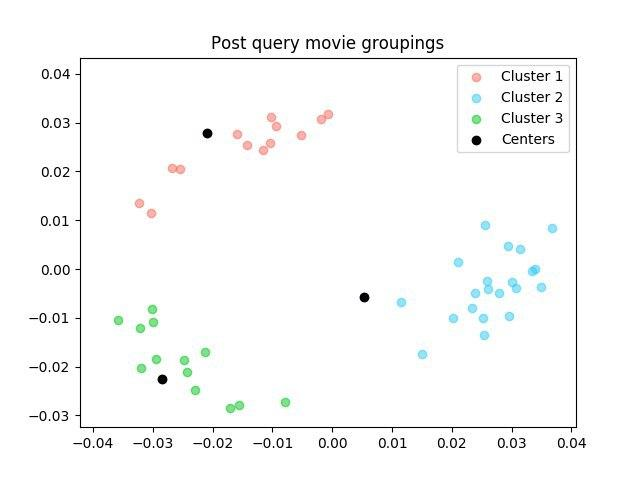
\includegraphics[width=9cm]{images/image1.jpg}
  \caption{Post-query results for ``Star Wars'' clustered using K-Means++.}
  \label{fig:clusters}
\end{figure}

As we tried using the HAC algorithm, we quickly realized the difficulty of deciding how many k-clusters should be used on each query. We found this to be extremely difficult because of how hard it is to compute the costs in this algorithm, which is needed to determine k.

From this point on, we decided to stick with the K-Means++ model. We were able to compute the costs and generate ``elbow plots'' that plotted the cost over the number of k-centers. We wanted to do this dynamically so that the perfect number of clusters was used for every individual query. We again found this extremely difficult because the data returned changes with each query, meaning the number of clusters changes with each query. Though we can determine the number of clusters from an elbow plot, we could not successfully find the best way to determine when the number of clusters converged to a reasonable number on the fly. We decided to generate a sequence of queries and look at the plots and determine a hard-set value for the number of clusters. We ultimately found that in almost every case, the best number of clusters was 3. Fig. \ref{fig:clusters} displays the resulting clusters from a users query.

\section{Program Architecture}
The overall architecture of our program has five components: dataset processing, python server, galago search, clustering, and front-end. The dataset processing component imports the movie dataset which is then used to match search results' document IDs with their appropriate movies. The purpose of the python server is to serve the front-end and process any query by interfacing with the galago search program and the clustering function. Galago search performs the search on the movie dataset for a user query. The clustering function calculates and labels the clusters by using the search results returned from galago search. Finally, the front-end gets a query from the user and displays the search results and the clusters returned from the server. The flow of the program is shown in Fig. \ref{fig:arch} below.

\begin{figure}[h]
  \centering
  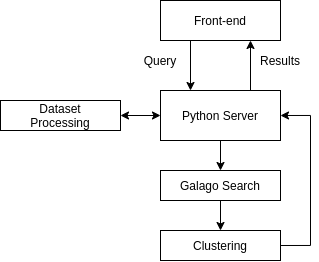
\includegraphics[width=6cm]{images/image2.png}
  \caption{Movie dataset search engine architecture.}
  \label{fig:arch}
\end{figure}

\section{Results}
Evaluating our relevance and clustering models was proving to be difficult due to our dataset being a combination of three different datasets. There were a couple of challenges we encountered. The first challenge was to create a qrels file for our relevance model. The second challenge was to use the Misra-Gries algorithm to evaluate the clusters generated by the models. Finally, we implemented a user interface for allowing users to make a query and visualize the search results and their clusters.

\subsection{Evaluating relevance model}
Since our dataset did not provide a qrels file, we decided to create our own. Since qrels is considered the ``correct answers'' for a particular query created from human judgement, we decided to create a qrels file for the query ``Star Wars'' \cite{qrels}. This process involved going through movies documents and marking their relevance to the query. However, we have more than 80,000 movies in the dataset. Rather than going through all of the movies, we scanned roughly 320 movies that were similar to ``Star Wars.''

\begin{center}
  \begin{table}[h]
    \caption{\label{tab:table1} MAP \& nDCG Results}
  \begin{tabular}{||c || c | c | c | c | c ||}
    \hline
     & \textbf{Title} & \textbf{Director} & \textbf{Actors} & \textbf{Desc.} & \textbf{Genre} \\ [0.5ex] 
    \hline\hline
    \textbf{MAP} & 0.30139 & 0.27874 & 0.27874 & 0.27680 & 0.25265\\ [0.5ex]
    \hline
    \textbf{nDCG} & 0.48531 & 0.47364 & 0.47364 & 0.47269 & 0.44456 \\ [0.5ex] 
    \hline
  \end{tabular}
  \end{table}
\end{center}

Once the qrels file was ready, we evaluated our model with MAP and nDCG. As we have mentioned earlier to prevent skewing from the reviews, our relevance model had five different weighting schemes. The five weighting schemes were for title, director, actors, description, and genre. Table \ref{tab:table1} below shows the results of MAP and nDCG for these five weighting schemes. As we can see since the query is ``Star Wars'', the weighting scheme that favored the title feature has the best results compared to the other four.

\subsection{Evaluating clustering model}
Our goal was to put the search result movies that were similar into the same cluster. To evaluate, we need a way to label the clusters. Thus, we used the Misra-Gries algorithm to find the most frequent terms in the genre feature of the clustered movies. Misra-Gries returns a specified number of frequent terms in a list. We choose to set the size of this list for the algorithm to ten. Table \ref{tab:table2} below shows the top five frequent terms for the clusters shown in Fig. \ref{fig:clusters} above.

\begin{center}
  \begin{table}[h]
    \caption{\label{tab:table2} Clusters with their lables}
  \begin{tabular}{||c || c ||}
    \hline
    \textbf{Clusters} & \textbf{Lables} \\ [0.5ex] 
    \hline\hline
    \textbf{Cluster 1} & Action, Adventure, Drama, Comedy, Biography \\ [0.5ex]
    \hline
    \textbf{Cluster 2} & Adventure, War, Romance, Action, Comedy \\ [0.5ex] 
    \hline
    \textbf{Cluster 3} & Adventure, Action, Drama, Fantasy, War \\ [0.5ex] 
    \hline
  \end{tabular}
  \end{table}
\end{center}

\subsection{User interface}

\begin{figure}[h]
  \centering
  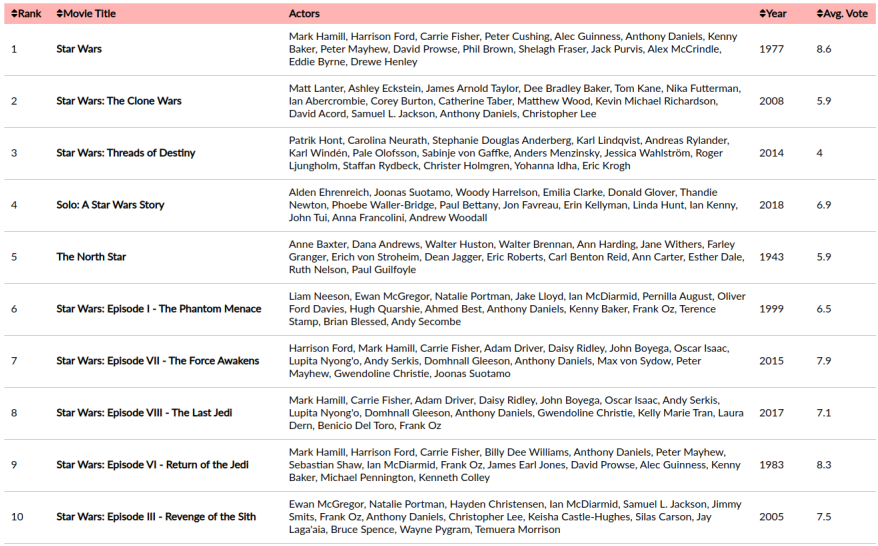
\includegraphics[width=8cm]{images/image3.png}
  \caption{Movie results returned from Galago Search with custom weights.}
  \label{fig:results}
\end{figure}

The last major part of our project was to have the results be displayed in a meaningful way to a user. This required displaying the biggest features of the movies returned from a search request along with displaying the clusters of similar movies. In order to achieve this, we created a user interface using HTML, Javascript, D3, and JQuery. This interface allowed a user to make a query via a search bar and dynamically display the results of that query. Fig. \ref{fig:results} above shows the results for the query ``Star Wars.'' Fig. \ref{fig:clusters_list} below shows the clusters of similar movies for the query ``Star Wars.''

\begin{figure}[h]
  \centering
  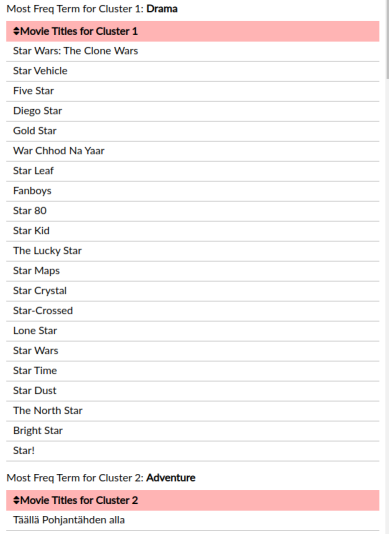
\includegraphics[width=6cm]{images/image4.png}
  \caption{List of movies clustered with labeled genre.}
  \label{fig:clusters_list}
\end{figure}

\section{Contribution}
With a team of three, this project was broken into three parts. Brandon was responsible for processing the data, converting the data to TREC format, creating an index for working with galago, and implementing the relevance model. Blaze was responsible for using the dataset with the Word2Vec library and responsible for developing the clustering models for post-query results. Raj was responsible for creating a web server, interfacing the front-end with the back-end server, interfacing back-end with galago program, and creating a user interface with web tools. 

\section{Conclusion}
Our goal was to create a search engine that also used clustering techniques to present post-query documents in a meaningful and easy to understand format. We explored topics covered in the Introduction to Information Retrieval class (CS 6550) such as relevance models, ranking algorithms, clustering, and evaluation metrics. We believe that the project ended up being a success. With more time, we believe that we could generate the number of clusters for any query dynamically so that the clustering model could improve its performance even more.

\bibliographystyle{ACM-Reference-Format}
\bibliography{bib/ref.bib}

\end{document}
\endinput
